%Directional Lead: Sven Vahsen

\subsubsection{Classes of Directional Detectors}
  
The various strategies for directional recoil detection are reviewed in Ref.~\cite{Vahsen:2021gnb}, and summarized in Fig.~\ref{directional_classification}. Directional detection can be achieved either directly by imaging the nuclear recoil trajectory, or indirectly by inferring the direction from a proxy variable. We will see below that low-density gas TPCs are capable of direct recoil imaging. Examples of the indirect approach include anisotropic light yield in crystals, and anisotropic ionization detection due to columnar recombination in liquid or gas. While the use of solid or liquid targets enabled by indirect techniques at first appears preferable to the gas TPC approach, in order to maximize target mass, to date none of the indirect effects have been clearly observed observed at the low, keV-scale, energies relevant for DM searches.  With a small (order 1\%) effect indirect effect, a prohibitively large number (order $10^5$) of DM interactions would be required to conlusively detect the DM dipole signal~\cite{Vahsen:2021gnb, OHare:2020lva}. Furthermore, indirect directionality typically does not yield independent event-level energy and direction information. That is a disadvantage, as DM detectors that do measure energy and direction independently, can serve the dual purpose of detecting solar neutrinos and reconstructing the incoming neutrino energies event-by-event from the recoil energies and directions. Another draw-back of the indirect method is reduced particle identification (and hence background rejection performance) because less information about the recoil is obtained. For all these reasons, the community working on directional detection is now focusing on detectors where the recoil direction is measured directly, at the event level, by imaging the recoil track. We refer to such detectors as Recoil Imaging Detectors~\cite{SnowmassIF53}.


\begin{figure}[!htbp]
\begin{center}
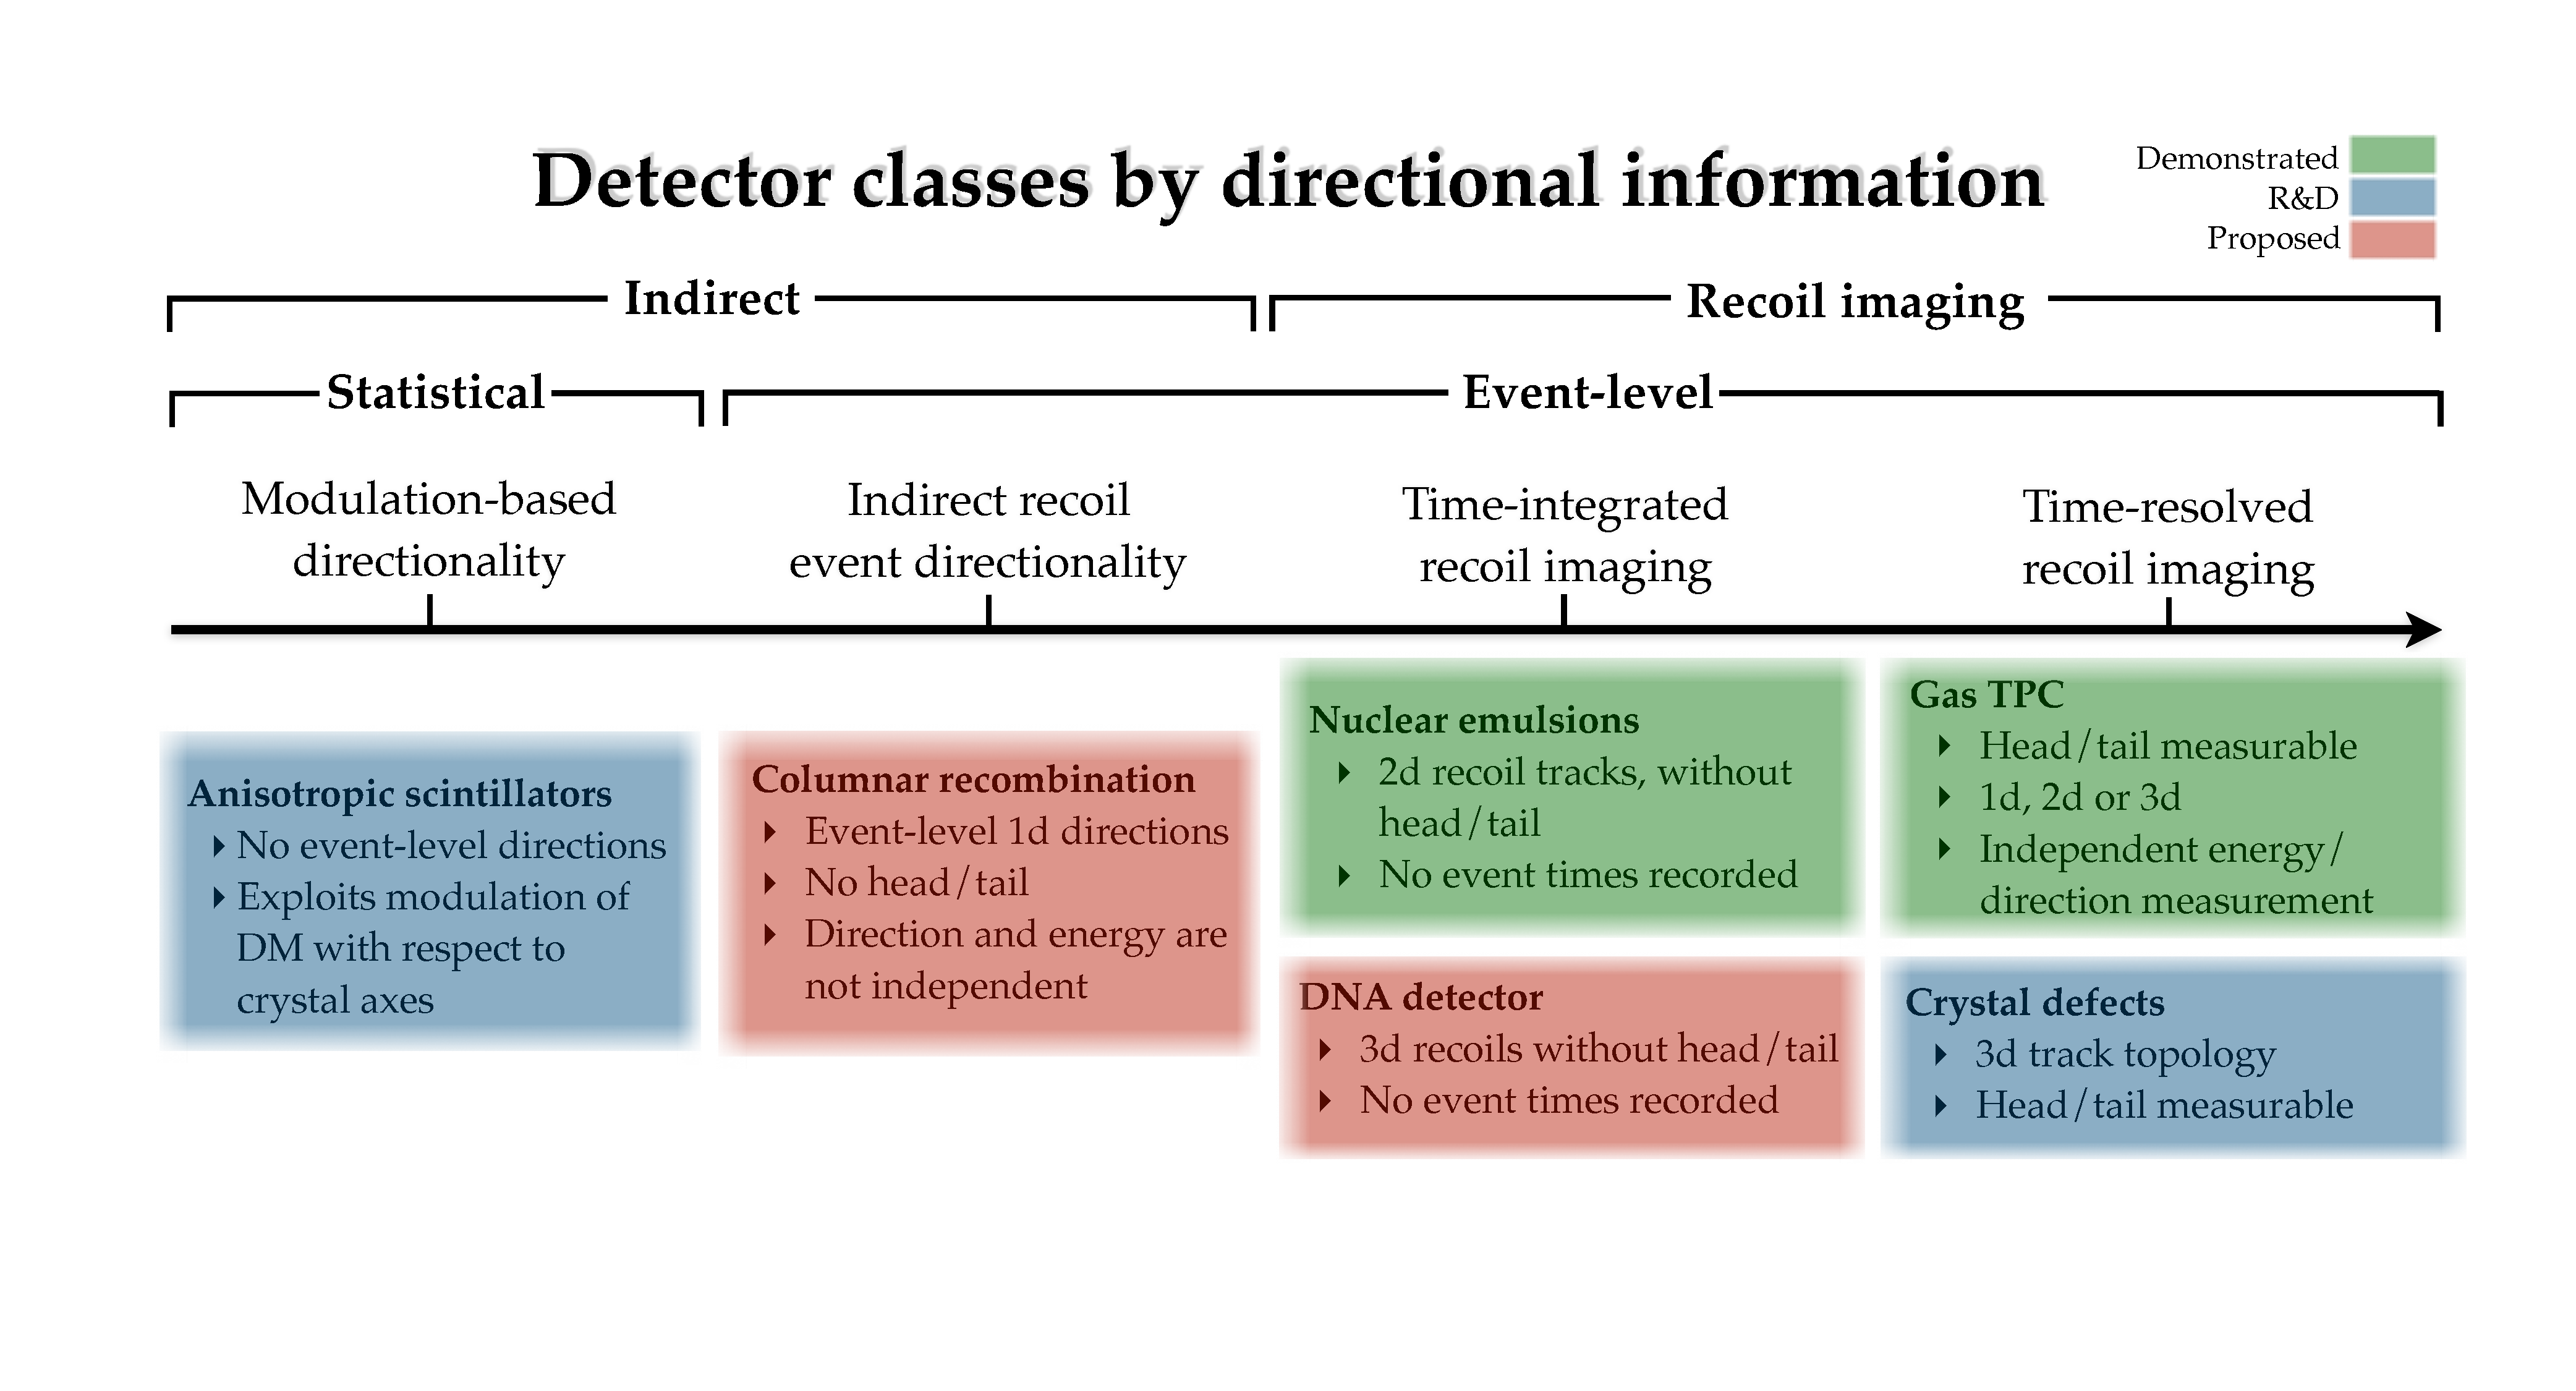
\includegraphics[width=0.99\columnwidth]{figures/DetectorClassTableAR.pdf}
\caption{ Figure adapted from Ref.~\cite{Vahsen:2021gnb}}\label{directional_classification}
\end{center}
\end{figure}

\subsubsection{Directional Detection Performance Requirements}
 
With a recoil-imaging detector, it is possible to observe the directional galactic dipole signature with as few as 5-10 detected DM events. The exact number of events required depends strongly on the detector’s directional performance. For example, to reject a solar neutrino background hypothesis at 90\% C.L., using only the observed angular distribution of recoils, requires less than 10 detected DM events if the performance is at the level of the following or better:

\begin{itemize}
\item recoil axis angular resolution $\leq 30^\circ$ 
\item efficiency for correctly detecting the recoil head/tail $>$ 80\%
\item offline rejection of electron-recoil background by factors $>10^5$. (Estimate for a 1000~${\rm m}^3$ gas TPC~\cite{Vahsen:2020pzb}. For smaller detectors, proportionally smaller rejection factors suffice.
\item fractional energy resolution, $\sigma_E/E$ of order 10\% at 5.9~keV
\item modest timing resolution, of order 0.5~h
\end{itemize}

The key technology challenge in directional detection is to meet the first three requirements at the lowest recoil energy possible, so that the required number of directional events can be detected with the smallest possible exposure.

\subsubsection{Recoil Imaging Technologies}
 
Detecting the direction of low-energy nuclear recoils at this level of accuracy is challenging. In condensed matter, the recoil length scale is order nm. In liquid TPCs where recoil ionization is drifted, electron diffusion is much larger than this recoil length and destroys the directional information. In solid targets, nuclear emulsions have been demonstrated as a means to achieve directional recoil detection. These detectors do not meet the timing requirement stated above, so that event time could not be used to transform the recoil direction into galactic coordinates. Such detectors would therefore have to be mounted on equatorial mounts, continuously rotating the detector to point towards the DM wind, so that the recoil direction always is with respect to the expected dipole direction. This complicates the detector design but is not an inherent showstopper. The NEWS collaboration (based in Japan and Italy) is pursuing directional recoil detection in emulsions~\cite{NEWS:2016fyf} and making good progress. Outside the particle physics community, defect spectroscopy in crystals~\cite{Marshall:2020azl} has been proposed as an alternative method for achieving directionality in solid targets. This work is at the early R\&D stage and would first need to be demonstrated as a viable technique for directional dark matter detection before it can gain traction in particle physics. The remaining world-wide groups working on recoil imaging are therefore pursuing low-density gas TPCs, which they consider the most promising direction. In gas TPC detectors, keV-scale nuclear recoils can be mm in length, while charge diffusion is of order 100~$\upmu$m. This allows the ionization from low-energy nuclear recoils, and hence recoil directions, to be reconstructed in detail. Recently, virtually all of the groups worldwide that are pursuing directional detection in gas TPCs joined forces to form the CYGNUS Detector R\&D collaboration.

\subsubsection{Quantum defects in wide-bandgap semiconductors}
 Quantum defects in wide-bandgap semiconductors are also proposed to achieve directional sensitivity at solid-state densities \cite{Rajendran:2017ynw,Marshall:2020azl, the snowmass whitepaper}. Event registration under this proposal would use technologies developed for DM detection in semiconductor targets, which yield the event time and mm-scale position. The incident particle's direction would be stored as a durable, submicron track of crystal lattice damage, which could be mapped using solid-state quantum sensing methods. Early R\&D has focused on nitrogen-vacancy defects in diamond \cite{Marshall:2020azl,Marshall:2021kjk,Marshall:2021xiu} to establish the feasibility of directional readout of such tracks. If successful, this will motivate further collaboration between the particle physics and solid-state quantum sensing communities toward DM detectors with sensitivity below the neutrino fog.
 
\subsubsection{CYGNUS}
 
The CYGNUS collaboration proposes to build a $\ge 1000~{\rm m}^3$ recoil-imaging gas target TPC. The proposed detector consists of a large number of smaller modules, which allows for the large volume to be distributed across multiple underground laboratories. Gas detectors have lower target mass per unit volume than liquid or solid target detectors, which is a clear disadvantage for DM searches. However, modern gas TPCs can detect even individual electrons of ionization with $\mathcal{O}(100~\upmu$m) spatial resolution, which is shorter than the nuclear recoil length, and enables directionality. Gas TPCs can be scaled to large volumes at reasonable cost without degrading performance, by using a modular structure where each module has a short, $\mathcal{O}$(50 cm), drift length. The unique directional capabilities of gas TPCs may outweigh their low target density once their cost is reduced sufficiently, when irreducible backgrounds appear, or if other physics can be performed. All three of these conditions are now met: 1) In recent years, micro-pattern gaseous detectors (MPGDs), developed by the RD51 collaboration at CERN for LHC experiments, have greatly reduced the cost of highly segmented TPC charge readout planes. As a result, recoil imaging gas TPCs are now realistic at a cost of order \$10k per cubic meter. This means even a 1000~m$^3$-scale observatory is at the \$10M cost scale, i.e. of similar cost as that of a single detection system in a large particle physics experiment. 2) We are rapidly approaching the neutrino fog, so that DM detectors are guaranteed to see an irreducible background. This is a background which can be clearly separated from DM signals via directionality. 3) The neutrino scattering events expected in the neutrino fog can also be exploited as a signal. Interestingly, already a much smaller, order 10~m$^3$ TPC module can do interesting solar neutrino measurements by also utilizing electron recoils. For a given neutrino energy, the electron recoils have much higher recoil energy but lower ionization density than nuclear recoils, and are readily observable in a low-threshold gas TPC, with directionality.

\begin{figure}[!htbp]
\begin{center}
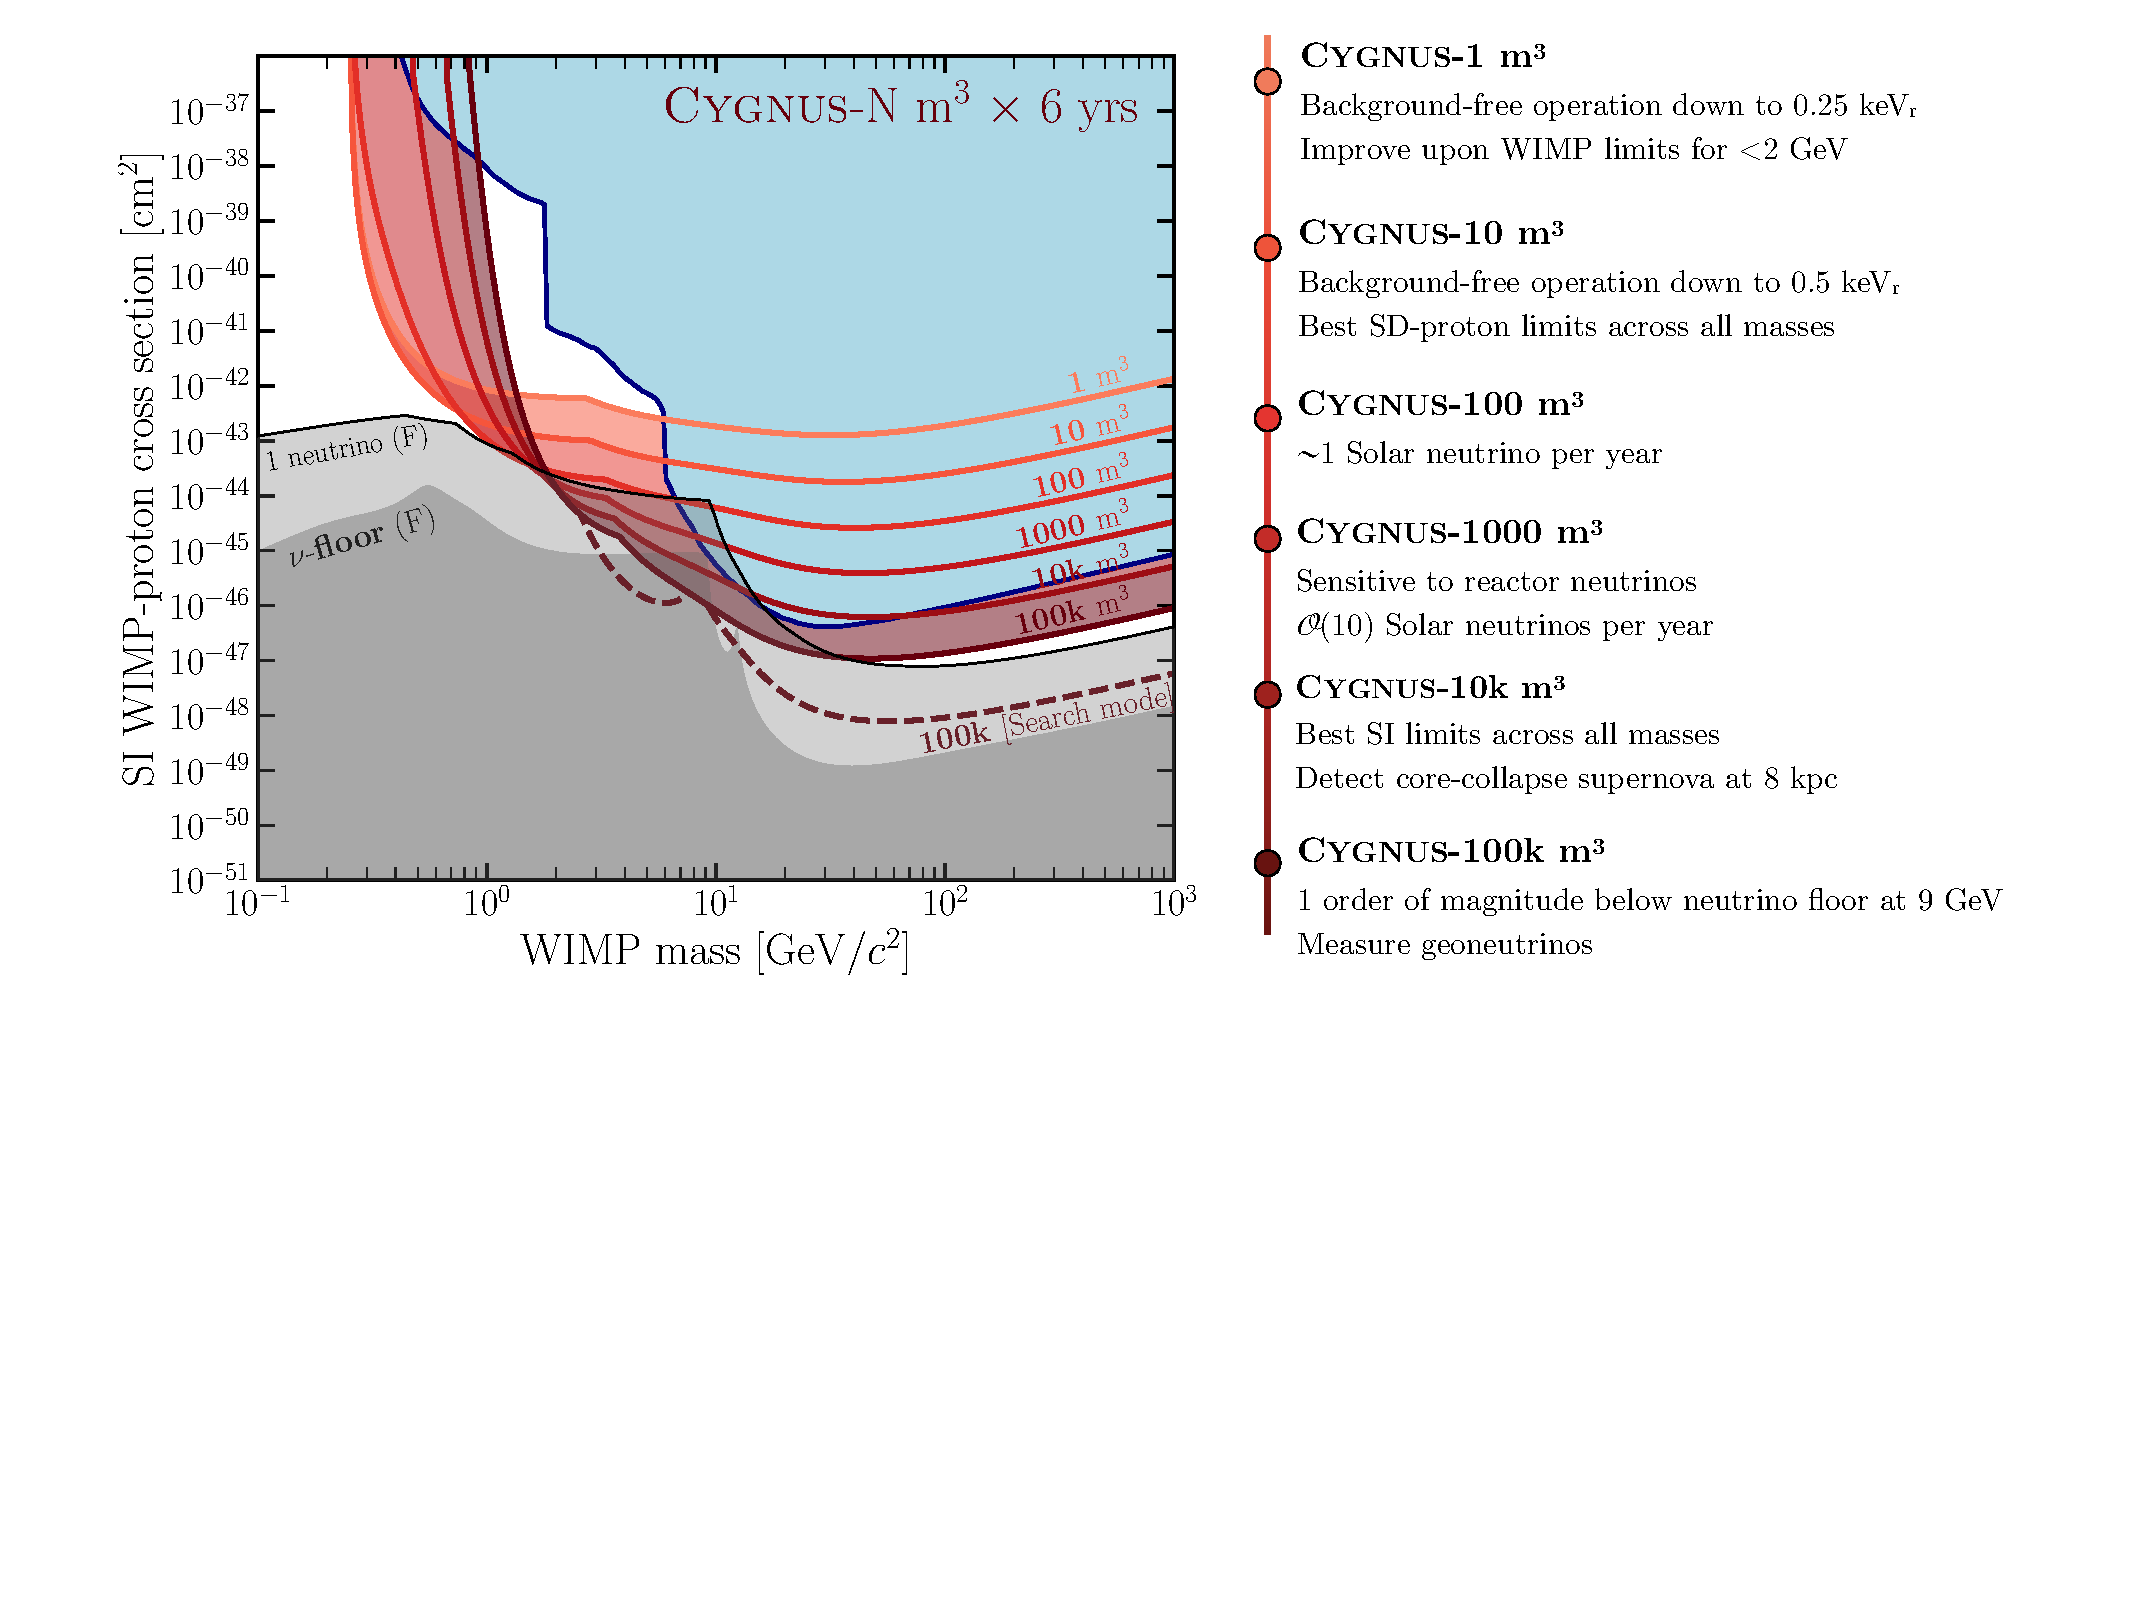
\includegraphics[width=0.99\columnwidth]{figures/Cygnus_listed_timeline.pdf}
\caption{Projected SI WIMP-proton scattering cross section 90\% CL exclusion limits for various CYGNUS fiducial volumes, each for 6 years of exposure, for a He:SF$_6$ (755 Torr : 5 Torr) fill gas. Currently excluded limits on the SI DM-nucleon cross section are shaded blue. The CYGNUS thresholds are increased evenly from 0.25 to 8 keVr for each increasing volume to reflect the range of possible thresholds of the final experiment. There is a factor 30 reach improvement possible if a non-directional ``search mode" fill gas such as 1520 Torr of SF$_6$ is used. We show this only for the largest scenario, but this option exists at every scale. Figure adapted from \cite{Vahsen:2020pzb}.\label{cygnus_timeline}}
\end{center}
\end{figure}

A plethora of other physics can be performed with a modest-volume, high-resolution gas TPC experiment. The staged program above will provide both competitive measurements of known phenomena, such as solar neutrinos, and unique searches for physics beyond the standard model, in the form of particle dark matter or non-standard neutrino interactions.  More details, including additional DM reach curves and expected neutrino event counts, can be found in a designated Snowmass White Paper~\cite{SnowmassIF53}, in a recent review of the field~\cite{Vahsen:2021gnb}, and in a concept paper describing the proposed CYGNUS experiment~\cite{Vahsen:2020pzb}. Figure~\ref{cygnus_timeline} shows the directional CYGNUS DM reach versus volume, for the potential target gas He:SF$_6$ (755 Torr : 5 Torr). Because the design and gas choice are not final, these reach curves are likely to change, possibly substantially, in the future.


%FIXME add #expected neutrino events here for some example gases?

The approximate timeline for CYGNUS worldwide is:
\begin{itemize}
\item 2022-2025: 1~m$^3$ detectors to be constructed and start operation in the UK, Japan, Italy, US, and Australia. The US detector may be used above-ground for CE$\upnu$NS measurements at a neutrino beam.
\item 2025-2035: 10~m$^3$ detectors: CYGNUS HD10 module (electronic readout) to be jointly constructed + operated in the US. A CYGNO detector (optical readout) program is planned and funded in Italy. Detectors in Japan, the UK, and Australia are also planned.  
\item 2024-2042+: 1000~m$^3$ detectors: design of $\ge$1000~m$^3$ facility with 10~m$^3$ modules to start in 2024. If the project remains successful, construction of a 1000~m$^3$ facility will begin in 2030.
\end{itemize}

\paragraph{CYGNUS HD in the US: Recoil Directionality below 10~keV}

The largest directional DM detector prototypes to date have been 1~m$^3$ in volume, and were built by the DRIFT and DMTPC collaborations. These early efforts were important in exploring two main approaches to the target gas, negative ion versus electron drift, and to the TPC readout, electronic versus optical. Both detectors were designed to search for 100-GeV DM particles, and have limited directionality for recoil energies below 50~keVr. Several hundred detected events would be required for a directional DM discovery with DRIFT. Recently, however, smaller R\&D detectors in the US have shown that the particle identification and event-level recoil directionality required for a directional discovery with only 5-10 events can be achieved even at sub-10-keV energies with modern MPGD-based detectors.

\begin{figure}[!htbp]
\begin{center}
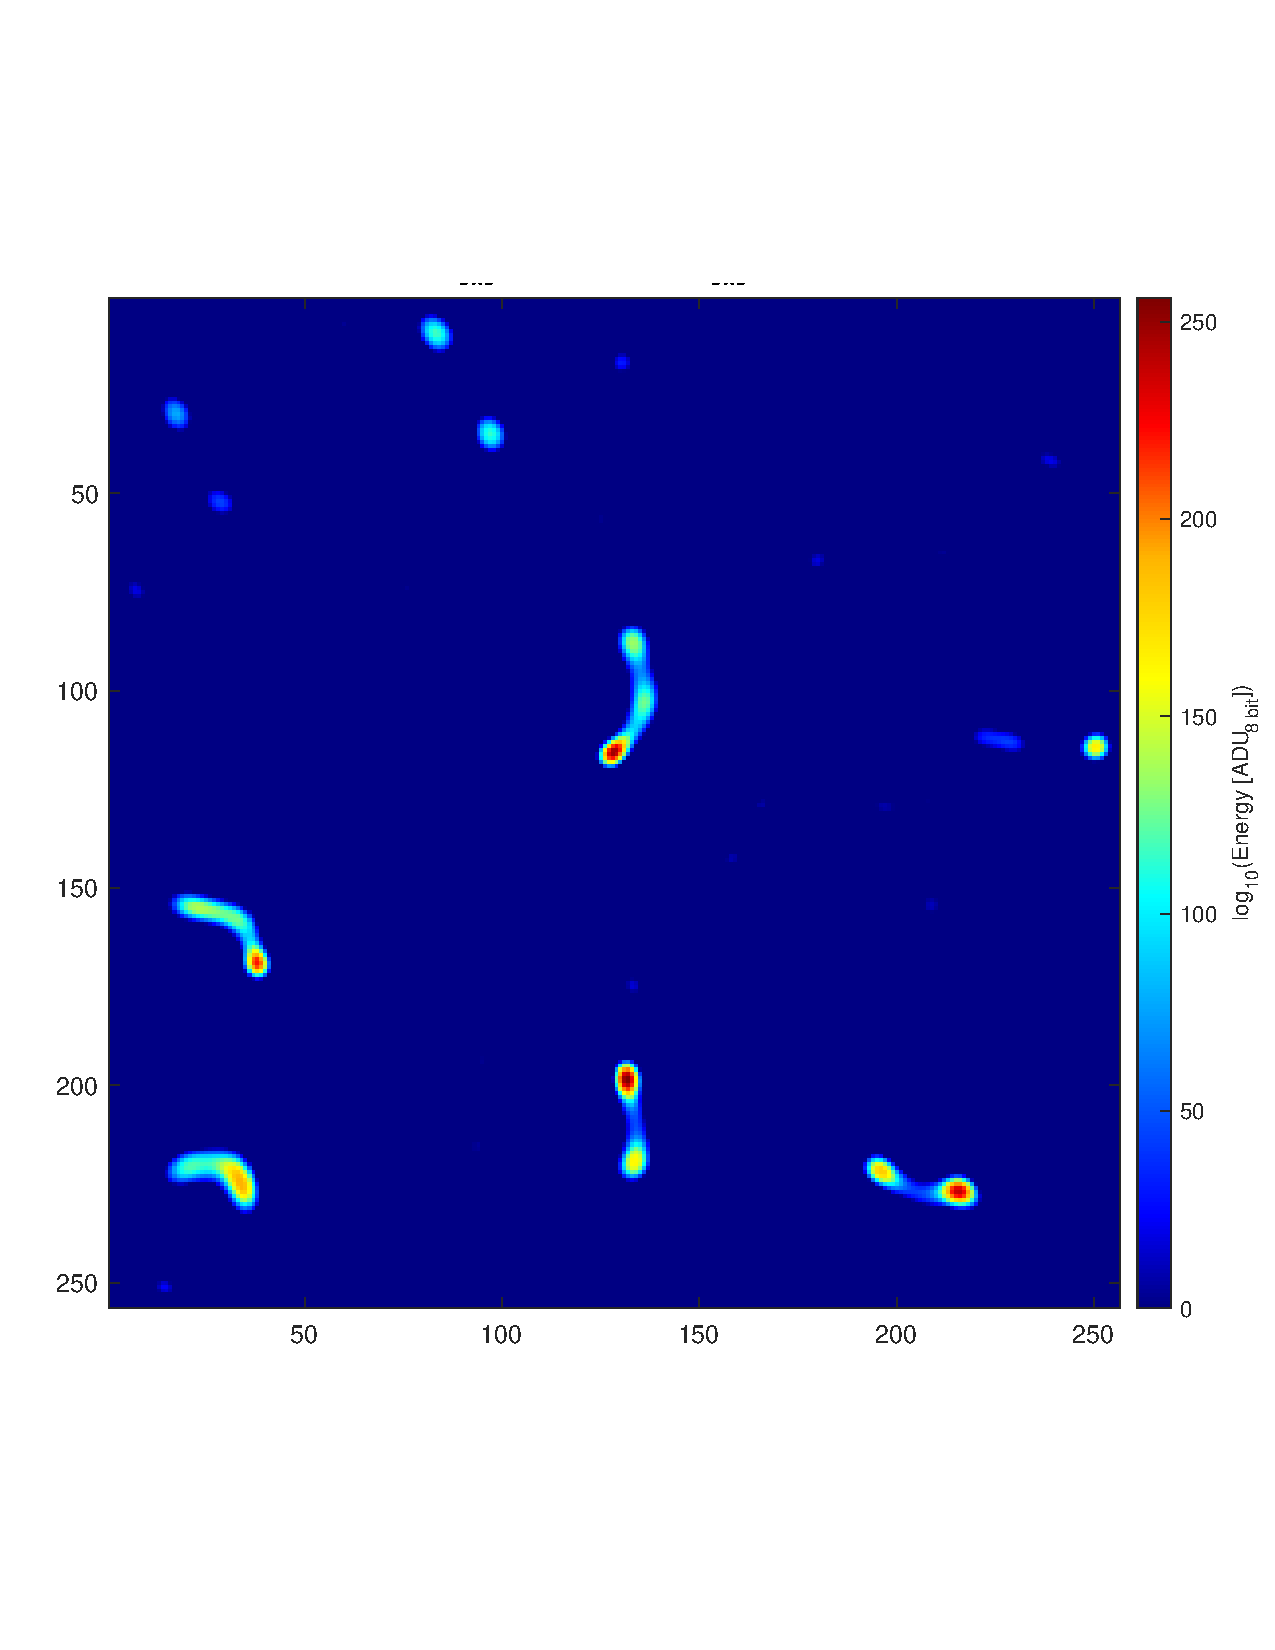
\includegraphics[width=0.49\columnwidth]{figures/optical_Fe55.pdf}
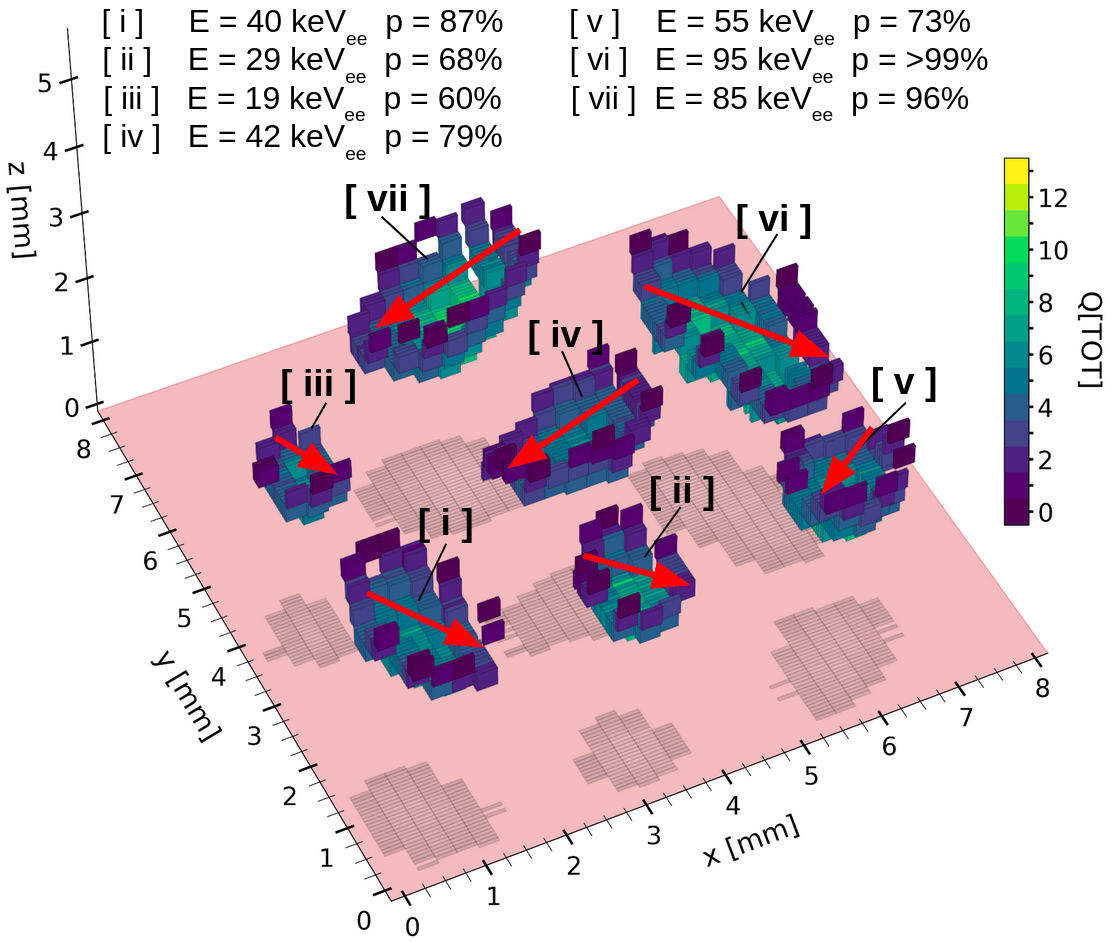
\includegraphics[width=0.49\columnwidth]{figures/BEAST_logain.png}
\caption{Experimental data from TPCs with MPGD readout. Left: 5.9~keV electron events in a 2D optical-readout TPC with GEM amplification at U. New Mexico. The fill gas is 30 Torr CF$_4$, the drift length is 2~cm, the gain $10^5$, the pixel size is $175 \times 175~\upmu$m$^2$. Deconvolution has been applied. Right: Helium-recoils induced with a neutron source, in a 3D electronic-readout TPC with GEM amplification at U. Hawaii. The fill gas is 760 Torr He:CO$_2$ (70:30), the drift length is 11~cm, the gain is ~$900$, the 3d voxel size is $50 \times 250 \times 250~\upmu$m$^3$. Raw data is shown, without any post-processing. The red arrows show fitted recoil directions, with the head and tail (i.e. sign of the vectors) determined by a 3d convolutional neural network. The confidence level of correct assignment is indicated in the legend. }\label{gas_tpc_events}
\end{center}
\end{figure}

Figure~\ref{gas_tpc_events} shows examples of electronic and nuclear recoil events recorded in state-of-the art ``CYGNUS HD'' TPC prototypes at US institutes. Advantages of optical readout include high segmentation and off-the-shelf, commercially available DAQ systems. Pixel ASIC readout is the most sensitive gas TPC readout technology, and enables 3d imaging. The events shown in Fig.~\ref{gas_tpc_events} (right) were recorded at low gain, only about 900, where electron recoils are strongly suppressed due to their lower ionization density. However, these detectors~\cite{Jaegle:2019jpx} operate stably at gains of at least $5\times 10^4$. Depending on the charge threshold used, at gains exceeding 3000-9000, single electrons of primary ionization are detected with high efficiency. Events recorded in single-electron mode are shown in Figure~\ref{single-electron}. The ionization threshold in this case is order 30~eV, and Sub-10-keV recoils are easily detectable as large signals compared to a negligible background from noise hits.


\begin{figure}[!htbp]
\begin{center}
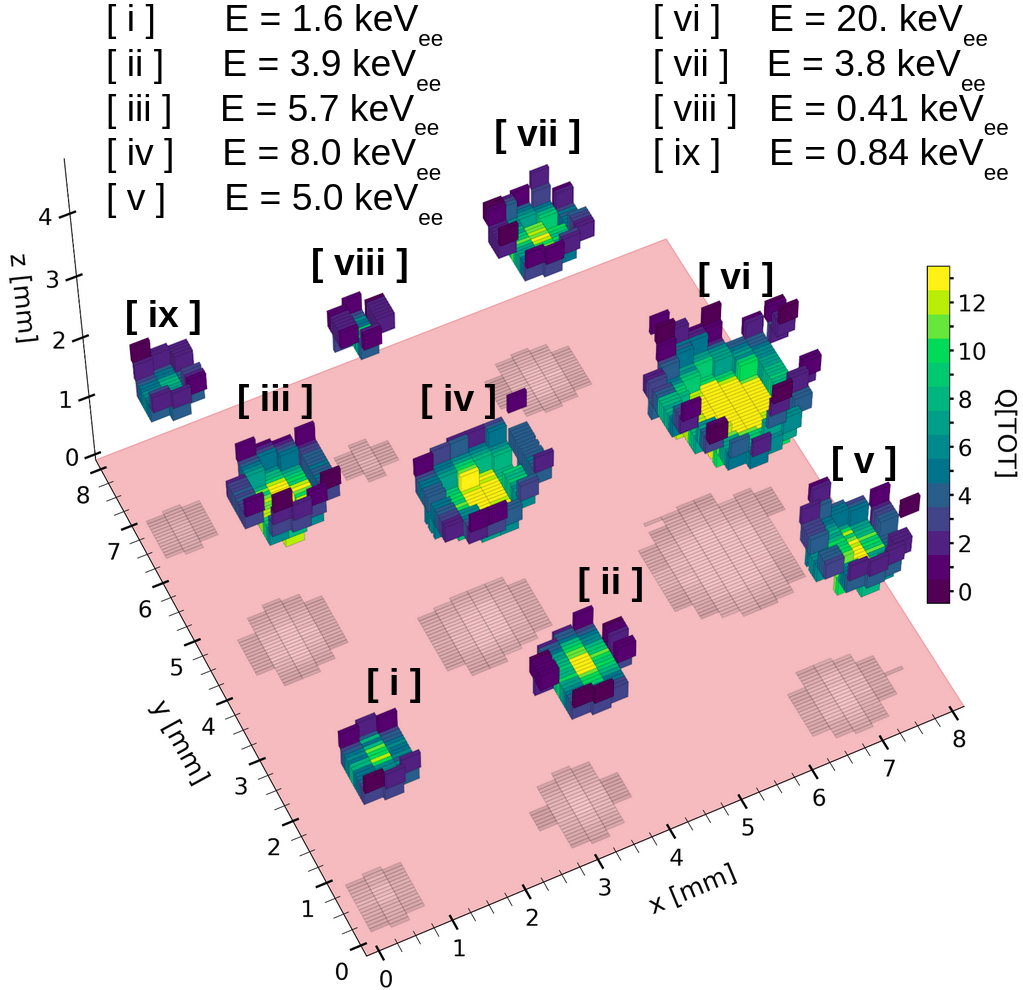
\includegraphics[width=0.49\columnwidth]{figures/BEAST_higain.png}
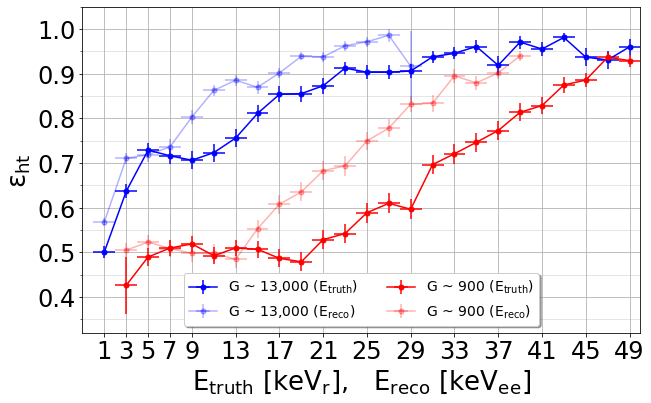
\includegraphics[width=0.49\columnwidth]{figures/headtail.png}
\caption{Left: Nuclear recoils detected in a pixel-ASIC TPC operating in the single-electron regime, at a gain of $1.3\times 10^4$. Right: Head/tail efficiency for helium-recoils versus energy, obtained with 3D convolutional neural networks on simulated pixel-ASIC TPC data for two different gas avalanche gain settings. }\label{single-electron}
\end{center}
\end{figure}

To utilize this type of extreme sensitivity in directional DM searches, the detectors themselves are not sufficient. We must also separate electronic and nuclear recoils, and assign recoil directions, even at the lowest observed energies. This challenge has motivated novel algorithm development for low-energy particle identification and head/tail detection over the last few years. CYGNUS HD recently achieved both the desired low-energy particle identification and directional capabilities with 3D convolutional neural networks (3D CNNs). Figure~\ref{single-electron} right shows the head/tail correct assignment efficiency in a pixel TPC, versus recoil energy. At low gain (\~900), the desired 70\% head/tail efficiency is obtained only down to 20~keVee in simulation, while in high-gain (single-electron) mode, this performance is extended down to 3keVee. The low-gain performance has already been confirmed experimentally. The high-gain experimental data is currently being analyzed.

These recent developments are extremely promising. However, we expect substantial further improvements: the event displays and 3~keVee directional threshold seen in Fig.~\ref{single-electron} is obtained with an electron drift (i.e. high diffusion) gas at atmospheric pressure. Both choices reduce low-energy directionality. Also, the detector utilizes a double-GEM gain stage which limits the point resolution. The result is that the sub-10~keV recoils appear round to the eye, even though the CNN can still determine the head/tail in this regime. A CYGNUS feasibility study~\cite{Vahsen:2020pzb} suggested that Micromegas amplification integrated with 2D x/y strip readout is a cost-optimal way to improve the low-energy performance even further, and to scale directional detectors up to very large volumes. Because of reduced charge sharing across fewer pixels in a micromegas-based detectors compared to GEM-based detectors, the gain required for single-electron detection is reduced by a factor of ~5. Then, it should be feasible to detect single electron even when using negative ion drift, where gains are reduced. The negative ion drift would in turn minimize diffusion, while the electron counting would remove the contributions of gain-fluctuations to the energy resolution. The expected end results would be a CYGNUS detector operating at the fundamental performance limit, where individual primary electrons are counted in 3d at $100~\upmu$m$^3$ spatial resolution. Recent R\&D with GridPix charge readout ~\cite{Ligtenberg:2021viw} has demonstrated the feasibility of this on a smaller scale. The CYGNUS HD members in the US are currently building prototypes to demonstrate sub-10-keV directionality at the 40~l and then 1000~l module scale. For further detail, we refer the reader to Refs.~\cite{Vahsen:2021gnb,Vahsen:2020pzb}. 



